\chapter{Dataset e simulazione degli scambi}
\label{chap_5}
Questo capitolo descrive il processo con cui è stato costruito il dataset utilizzato per l'addestramento, la validazione e il test del modello di deep learning presentato in questa tesi. I punti di partenza sono due database pubblici distribuiti da PhysioNet~\cite{goldberger2000physionet}, \textbf{PTB-XL}~\cite{wagner2020ptbxl} e \textbf{Georgia}~\cite{alday2020georgia}, da cui sono stati estratti i tracciati ECG grezzi. A partire da questi, il dataset finale è stato ottenuto tramite un'unica pipeline che elabora e combina entrambe le sorgenti. Organizzata in tre fasi logicamente distinte:

\begin{enumerate}
	\item la \textbf{suddivisione delle registrazioni} di ciascun database in insiemi di training, validazione e test, effettuata separatamente su PTB-XL e Georgia e poi unita, in modo da garantire che nessun paziente sia condiviso tra split diversi;
	\item la \textbf{segmentazione beat-by-beat} delle registrazioni, con lo scopo di isolare singoli battiti cardiaci in finestre temporali di dimensione fissa; il numero di battiti estratti per registrazione dipende dallo split di appartenenza;
	\item la \textbf{simulazione artificiale di scambi di elettrodi}, necessaria per generare esempi etichettati di posizionamento errato, dato che nessuno dei due database originali contiene annotazioni di questo tipo.
\end{enumerate}

Nei paragrafi seguenti vengono presentate le caratteristiche dei due database di partenza, motivate le scelte progettuali di ciascuna fase e descritta nel dettaglio la struttura del dataset finale. Un terzo database, utilizzato esclusivamente per una valutazione indipendente del modello, è presentato separatamente nella Sezione~\ref{sec:china_dataset}.

\section{Database di partenza}

\subsection{Il database PTB-XL}

PTB-XL è un database pubblico di ECG clinici a 12 derivazioni, pubblicato dal Physikalisch-Technische Bundesanstalt (PTB) e reso disponibile attraverso PhysioNet~\cite{wagner2020ptbxl}. Si tratta, ad oggi, di uno dei più grandi database ECG annotati liberamente accessibili, per questo motivo è ampiamente utilizzato come benchmark in letteratura per problemi di classificazione automatica di segnali cardiaci o patologie.

Ogni registrazione contenuta in PTB-XL è un ECG a riposo della durata di 10 secondi, acquisito con le 12 derivazioni standard (I, II, III, aVR, aVL, aVF, V1--V6). Il database mette a disposizione i segnali grezzi a due diverse frequenze di campionamento (100~Hz e 500~Hz), oltre a un insieme di metadati per ciascuna registrazione: dati demografici del paziente (età, sesso), diagnosi codificate secondo lo standard SCP-ECG, informazioni sulla qualità del segnale e sull'apparecchiatura di acquisizione, e un identificativo di \texttt{patient\_id} che collega più registrazioni allo stesso paziente, dove presenti.

Le caratteristiche principali del database sono riassunte nella Tabella~\ref{tab:ptbxl_caratteristiche}.

\begin{table}[htbp]
	\centering
	\caption{Caratteristiche principali del database PTB-XL~\cite{wagner2020ptbxl}.}
	\label{tab:ptbxl_caratteristiche}
	\begin{tabular}{@{}ll@{}}
		\toprule
		\textbf{Caratteristica} & \textbf{Valore} \\
		\midrule
		Numero di registrazioni ECG & 21\,837 \\
		Numero di pazienti & 18\,885 \\
		Durata di ciascuna registrazione & 10 secondi \\
		Derivazioni & 12 \\
		Frequenze di campionamento disponibili & 100~Hz e 500~Hz \\
		Formato dei segnali grezzi & WFDB \\
		Risoluzione & 16 bit, \SI{1}{\micro\volt}/LSB \\
		Annotazioni diagnostiche & Codici SCP-ECG \\
		Metadati demografici & Età, sesso \\
		Origine geografica & Germania (interferenza a \SI{50}{Hz}) \\
		\bottomrule
	\end{tabular}
\end{table}

Dal punto di vista pratico, il database è organizzato in due componenti principali:

\begin{itemize}
	\item una cartella contenente i segnali grezzi in formato WFDB, suddivisi in sottocartelle per intervalli di \texttt{ecg\_id}, disponibili sia a \SI{100}{Hz} (\texttt{records100/}) sia a \SI{500}{Hz} (\texttt{records500/}); in questo lavoro sono stati utilizzati esclusivamente i segnali a \SI{500}{Hz}.
	\item un file di metadati \texttt{ptbxl\_database.csv}, in cui ogni riga corrisponde a una registrazione e riporta, tra le altre cose, il percorso relativo ai file del segnale, l'identificativo del paziente e le diagnosi codificate.
\end{itemize}

Ai fini di questo lavoro, il database è stato utilizzato esclusivamente come sorgente di tracciati ECG, conassunti come correttamente acquisiti in assenza di annotazioni cliniche esplicite di malposizionamento, pur riconoscendo i limiti intrinseci legati alla potenziale presenza di rumore o errori sistematici latenti nelle registrazioni del mondo reale. Le diagnosi cliniche associate a ciascuna registrazione non sono state impiegate, poiché l'obiettivo del modello non è la diagnosi della patologia cardiaca, ma la verifica della corretta acquisizione del segnale stesso.

\subsection{Il database Georgia}

Il secondo database utilizzato è il \emph{Georgia 12-Lead ECG Challenge Database}, distribuito da PhysioNet e originariamente pubblicato come parte dei dati di training della PhysioNet/Computing in Cardiology Challenge 2020~\cite{alday2020georgia}. A differenza di PTB-XL, che rappresenta prevalentemente una popolazione europea, Georgia raccoglie registrazioni acquisite negli Stati Uniti sud-orientali, ampliando così la variabilità demografica e strumentale del dataset finale.

Ogni registrazione è un ECG a 12 derivazioni standard, campionato a \SI{500}{Hz}, distribuito in formato WFDB (coppia di file \texttt{.hea}/\texttt{.mat}). A differenza di PTB-XL, il database non fornisce un file di metadati tabellare separato: le informazioni su ciascuna registrazione (età, sesso, diagnosi codificate secondo SNOMED-CT) sono riportate direttamente nell'header \texttt{.hea} del singolo record, e ogni registrazione corrisponde a un paziente distinto (non esistono, cioè, più registrazioni associate allo stesso \texttt{patient\_id}, a differenza di PTB-XL). Le caratteristiche principali sono riassunte nella Tabella~\ref{tab:georgia_caratteristiche}.

\begin{table}[htbp]
	\centering
	\caption{Caratteristiche principali del database Georgia~\cite{alday2020georgia}.}
	\label{tab:georgia_caratteristiche}
	\begin{tabular}{@{}ll@{}}
		\toprule
		\textbf{Caratteristica} & \textbf{Valore} \\
		\midrule
		Numero di registrazioni ECG & $\sim$10\,300 \\
		Numero di pazienti & uno per registrazione \\
		Durata di ciascuna registrazione & 5 o 10 secondi \\
		Derivazioni & 12 \\
		Frequenza di campionamento & 500~Hz \\
		Formato dei segnali grezzi & WFDB \\
		Annotazioni diagnostiche & Codici SNOMED-CT \\
		Origine geografica & Stati Uniti (interferenza a \SI{60}{Hz}) \\
		\bottomrule
	\end{tabular}
\end{table}

Poiché il database non è distribuito con un unico indice tabellare, l'elenco delle registrazioni disponibili è stato ricostruito a partire dai file \texttt{RECORDS} presenti nelle varie sottocartelle del database, ciascuno dei quali elenca i nomi dei record contenuti al suo interno; i percorsi così ottenuti sono stati utilizzati per ricavare l'insieme completo e univoco delle registrazioni disponibili.

Come per PTB-XL, anche per Georgia sono stati utilizzati esclusivamente i tracciati grezzi, applicando le stesse assunzioni.

\subsubsection{Osservazione sull'ordine delle derivazioni e sul filtro di rete}

I due database, pur condividendo lo stesso insieme di 12 derivazioni standard, differiscono in due aspetti tecnici rilevanti per l'elaborazione:

\begin{itemize}
	\item l'ordine con cui le derivazioni sono salvate nei file WFDB è verificato esplicitamente in fase di caricamento, per evitare di associare per errore un canale alla derivazione sbagliata;
	\item poiché PTB-XL è stato acquisito in un contesto con interferenza della linea elettrica a \SI{50}{Hz} (Europa) e Georgia con un'interferenza di \SI{60}{Hz} (Stati Uniti), il filtro \emph{notch} applicato in fase di pulizia del segnale (Sezione~\ref{sec:preprocessing}) utilizza una frequenza di taglio diversa per le due sorgenti, così da rimuovere correttamente l'interferenza di rete in entrambi i casi.
\end{itemize}

\section{Pipeline di costruzione del dataset}
\label{sec:pipeline_overview}

La costruzione del dataset finale è realizzata da due script che elaborano PTB-XL e Georgia, in modo da ottenere con il primo script un dataset composto da segmenti beat-by-beat e preprocessati, mentre con il secondo applica le trasformazioni richieste dall'utente. Concettualmente, la pipeline è organizzata in tre fasi sequenziali:

\begin{enumerate}
	\item \textbf{Suddivisione in train/val/test}: le registrazioni di ciascun database vengono assegnate a uno dei tre split (descritto in dettaglio nella Sezione~\ref{sec:split}), in modo che tutte le registrazioni di uno stesso paziente ricadano nello stesso insieme.
	\item \textbf{Segmentazione beat-by-beat}: per ogni registrazione vengono individuati i picchi R e vengono estratte finestre temporali di durata fissa centrate su di essi, secondo criteri che dipendono dallo split di appartenenza (Sezione~\ref{beat-by-beat-segmentation}): due battiti per registrazione in train/val, tutti i battiti validi in test.
	\item \textbf{Simulazione degli scambi di elettrodi}: ai battiti di train e validazione viene assegnata un'etichetta, scelta tra "normale" e un insieme di scambi di elettrodi clinicamente plausibili, e i segnali vengono trasformati in modo coerente con l'etichetta assegnata (Sezione~\ref{sec:simulazione_misplacement}); i battiti di test restano invece invariati, etichettati come "normale".
\end{enumerate}

Questa suddivisione in due script permette di velocizzare il processo di creazione di dataset differenti (con trasformazioni diverse), in quanto le prime due fasi, comprese nel primo script, sono sempre uguali indifferentemente dal tipo di trasformazione che si vuole applicare al dataset.

\section{Suddivisione in training, validazione e test}
\label{sec:split}

La suddivisione in train/validation/test è il primo passo della costruzione del dataset, ed è pensata per evitare qualunque forma di \emph{data leakage} tra split diversi.

La suddivisione avviene a livello di \textbf{paziente} e non di singola registrazione o singolo battito: per \emph{PTB-XL}, dove uno stesso paziente può essere associato a più registrazioni (\texttt{ecg\_id} diversi), lo split è effettuato sull'insieme dei \texttt{patient\_id} univoci, così che tutte le registrazioni di uno stesso paziente vengono assegnate allo stesso split; per \emph{Georgia}, dove ogni registrazione corrisponde a un paziente distinto, lo split sull'identificativo di registrazione è equivalente, per costruzione, a uno split per paziente.

\subsection{Proporzioni e procedura}
Per ciascun database, gli identificativi vengono ordinati, mescolati con un generatore pseudo-casuale a seed fisso e suddivisi secondo le proporzioni: 80\% training, 10\% validazione, 10\% test, modificabili in caso di necessità dall'utente.

La suddivisione viene effettuata \textbf{separatamente} su PTB-XL e su Georgia, e successivamente i due risultati vengono uniti per formare gli split combinati finali; ogni split conterrà quindi una parte di registrazioni PTB-XL e una parte di registrazioni Georgia, nelle stesse proporzioni 80/10/10 calcolate all'interno di ciascun database. L'uso di un seed fisso rende la suddivisione riproducibile.

\section{Segmentazione beat-by-beat}
\label{beat-by-beat-segmentation}

La scelta di lavorare a livello di singolo battito, anziché sull'intera registrazione, è motivata da diverse considerazioni.

\begin{description}
	\item[Dimensione di input uniforme.] Il numero di battiti contenuti in una registrazione di durata fissa dipende dalla frequenza cardiaca del soggetto, che varia da paziente a paziente e nel tempo. Segmentare rispetto al singolo battito, anziché all'intera registrazione, permette di ottenere input di dimensione fissa e nota a priori, indipendente dalla frequenza cardiaca, semplificando l'architettura della rete e il relativo addestramento.
	\item[Aumento della numerosità campionaria (train/val).] Da ogni registrazione di training o validazione vengono estratti due segmenti, aumentando la numerosità del dataset a disposizione del modello, fattore particolarmente rilevante con architetture di deep learning.
	\item[Localizzazione del segnale informativo.] L'obiettivo del modello è riconoscere pattern morfologici legati al posizionamento degli elettrodi, come inversioni di polarità di alcune derivazioni o scambi di ampiezza tra derivazioni, che sono osservabili già a livello del singolo ciclo cardiaco. Non è quindi necessario fornire al modello l'intera registrazione per permettergli di apprendere pattern più complessi non utili in questo caso di studio; concentrare l'input sul singolo battito riduce la quantità di informazione ridondante che il modello deve elaborare.
	\item[Riduzione del costo computazionale.] Input più corti riducono il numero di parametri e le risorse di calcolo richieste, sia in fase di addestramento sia in fase di inferenza.
\end{description}

\subsection{Rilevamento dei picchi R}

Per individuare i battiti all'interno di ciascuna registrazione, è necessario innanzitutto localizzare i picchi R, cioè i picchi di ampiezza massima del complesso QRS, che costituiscono il punto di riferimento temporale più affidabile e riproducibile del ciclo cardiaco. Il rilevamento è stato eseguito tramite l'algoritmo di \textit{Pan-Tompkins}~\cite{pantompkins1985}.

Un aspetto progettuale rilevante riguarda la scelta della derivazione sulla quale eseguire il rilevamento. Sebbene il segnale a 12 derivazioni contenga, per ciascuna derivazione, una propria rappresentazione dello stesso ciclo cardiaco, il rilevamento dei picchi R non è stato effettuato in modo indipendente su ciascuna derivazione, ma su due \textit{derivazioni guida}, \textit{V1} e \textit{V5}, scelte perché tra loro elettricamente ortogonali e con una buona visione del complesso QRS.

L'algoritmo di Pan-Tompkins viene applicato separatamente a V1 e V5, ottenendo due liste di picchi candidati. Le due liste vengono poi accoppiate: per ogni picco rilevato su V1 si cerca, su V5, il picco più vicino entro una tolleranza fissata (50~ms); se un accoppiamento valido viene trovato, la posizione finale del picco R è ottenuta come media delle due posizioni accoppiate, altrimenti il candidato viene scartato. Questo accoppiamento, rispetto a una semplice media indipendente delle due liste, ha lo scopo di scartare rilevamenti isolati presenti su una sola delle due derivazioni guida, ad esempio dovuti a rumore residuo, e di garantire che il picco R utilizzato per la segmentazione sia effettivamente supportato da entrambe le derivazioni di riferimento. La medesima posizione temporale, così ottenuta, viene infine utilizzata per estrarre la finestra su tutte e dodici le derivazioni.

Questa scelta non è solo una semplificazione implementativa, ma è funzionale all'obiettivo della tesi: se il rilevamento dei picchi fosse eseguito derivazione per derivazione, uno scambio di elettrodi che alteri la morfologia di una specifica derivazione potrebbe causare un rilevamento del picco R leggermente disallineato rispetto alle altre derivazioni, introducendo nella finestra estratta un disallineamento temporale artificiale, dovuto al preprocessing e non alla reale anomalia di acquisizione. Questo problema rischierebbe di essere appreso dal modello come indicatore di misplacement, invalidando così l'esperimento.

\subsection{Estrazione della finestra}

Per ogni picco R rilevato, viene estratta una finestra temporale $[R - 400\,\text{ms},\ R + 600\,\text{ms}]$, per una durata complessiva di un secondo, sincronizzata su tutte le 12 derivazioni. La Figura~\ref{fig:finestra_segmentazione} illustra graficamente questa finestra su un battito di esempio.

\begin{figure}[htbp]
	\centering
	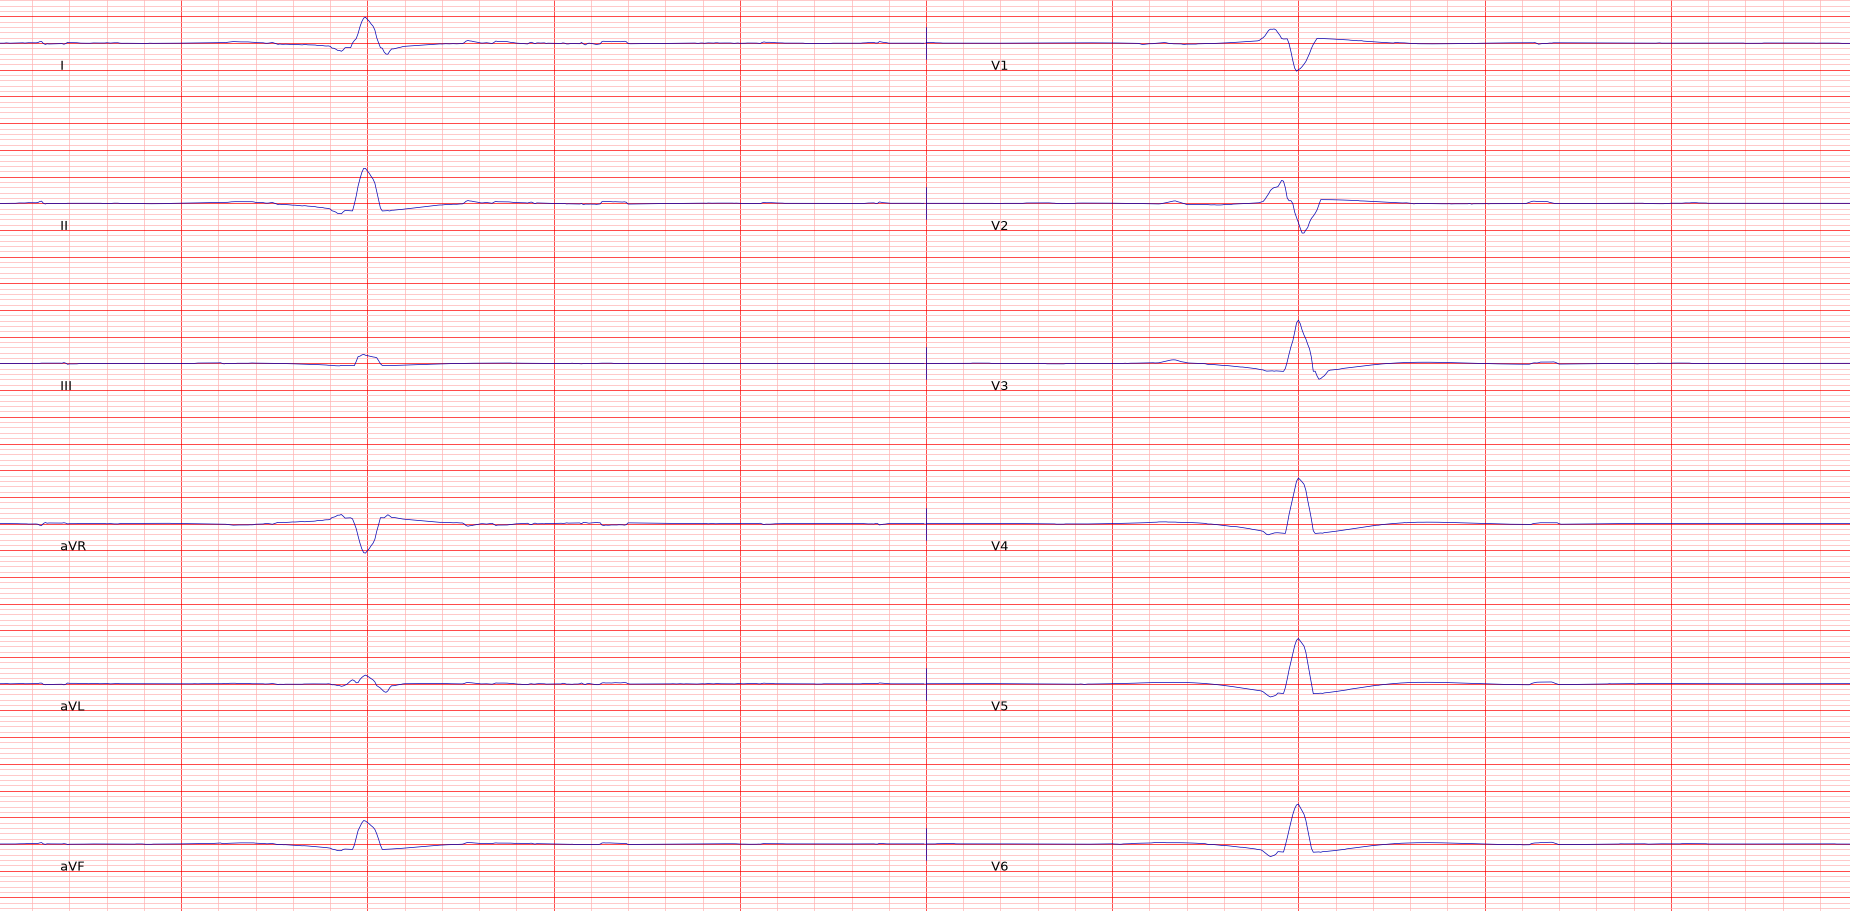
\includegraphics[width=\textwidth]{images/beat_segment.png}
	\caption{Finestra di segmentazione $[R-400\,\text{ms},\,R+600\,\text{ms}]$ centrata sul picco R, sovrapposta a un tracciato ECG di esempio.}
	\label{fig:finestra_segmentazione}
\end{figure}

La scelta di un'asimmetria tra la porzione precedente e quella successiva al picco R (400~ms prima, 600~ms dopo) è motivata dalla successione temporale delle componenti morfologiche dell'onda ECG all'interno di un singolo ciclo cardiaco:

\begin{itemize}
	\item i 400~ms che precedono il picco R sono sufficienti a includere l'onda P (depolarizzazione atriale) e il tratto PR, che hanno una durata tipica complessiva dell'ordine di circa 200~ms;
	\item i 600~ms successivi al picco R sono necessari a includere il resto del complesso QRS, il tratto ST e l'intera onda T (ripolarizzazione ventricolare), la cui durata complessiva, specialmente considerando l'intervallo QT, può arrivare fino a circa 400--450~ms in condizioni fisiologiche normali, con un margine di sicurezza per frequenze cardiache più basse (a cui corrisponde un intervallo QT più lungo).
\end{itemize}

Una finestra di un secondo, centrata in modo asimmetrico sul picco R, permette, nella grande maggioranza dei casi, di catturare un intero ciclo cardiaco (onda P, complesso QRS, onda T) senza includere porzioni significative del battito precedente o successivo, anche per frequenze cardiache elevate. Una finestra i cui estremi cadono fuori dai limiti della registrazione (tipicamente il primo o l'ultimo battito) viene scartata.

\subsection{Numero di battiti estratti: differenza tra train/val e test}
\label{sec:beat_count_per_split}

Il numero di battiti estratti da ciascuna registrazione dipende dallo split di appartenenza, poiché training/validazione e test hanno scopi diversi nella pipeline:

\begin{itemize}
	\item \textbf{Training e validazione}: da ogni registrazione vengono estratti esattamente \textbf{due battiti}: i primi e gli ultimi battiti di ciascuna registrazione di 10 secondi vengono deliberatamente evitati per eliminare l'influenza dei transitori di accensione, dei filtri analogici e degli effetti di bordo temporali introdotti dai filtri di preprocessing. La scelta del terzo e del quinto picco garantisce l'estrazione di cicli cardiaci stabili e interni alla registrazione tramite una procedura deterministica e riproducibile. Se una registrazione produce meno di cinque picchi R validi, essa viene scartata e registrata come tale (si veda la Sezione~\ref{sec:struttura_finale}). Questi due battiti sono poi la base su cui viene applicata la simulazione degli scambi di elettrodi (Sezione~\ref{sec:simulazione_misplacement}).
	\item \textbf{Test}: da ogni registrazione vengono estratti \textbf{tutti i battiti validi}, senza limitarsi a due. Questa scelta è funzionale alla strategia di valutazione adottata, poiché, in fase di test, ogni registrazione viene classificata tramite \emph{majority voting} sulle predizioni ottenute sui singoli battiti che la compongono, e disporre di più battiti per registrazione rende questa stima più robusta. I battiti di test non vengono sottoposti ad alcuna trasformazione e sono etichettati come ``normale'', poiché rappresentano registrazioni reali presumibilmente acquisite con un posizionamento corretto degli elettrodi.
\end{itemize}

\section{Simulazione degli scambi di elettrodi}
\label{sec:simulazione_misplacement}

\subsection{Perché è necessaria una simulazione}

I database di partenza, come la generalità dei database ECG pubblici, contengono esclusivamente registrazioni acquisite con un posizionamento corretto degli elettrodi: non esiste, nella pratica clinica, la produzione sistematica e su larga scala di registrazioni etichettate come ``mal posizionate'', poiché si tratta di un errore di acquisizione che, quando osservato, viene generalmente corretto immediatamente e non salvato. Per addestrare un modello supervisionato in grado di riconoscere queste condizioni, è quindi necessario disporre di esempi delle diverse classi di errore, e l'unica strada percorribile è la generazione artificiale di tali esempi a partire da registrazioni corrette. Questa simulazione viene applicata unicamente ai battiti di training e validazione (si veda la Sezione~\ref{sec:beat_count_per_split}); i battiti di test restano non trasformati.

Questo approccio è reso possibile dal fatto che il posizionamento errato di un elettrodo non introduce, dal punto di vista del segnale, un errore arbitrario, bensì un effetto ben determinabile e prevedibile, descrivibile a partire dalle equazioni che definiscono le derivazioni standard. È proprio questa proprietà che viene sfruttata per costruire la simulazione.

\subsection{Equazioni delle derivazioni standard}

Le sei derivazioni degli arti non sono misurate direttamente, ma calcolate a partire dai potenziali elettrici rilevati da tre elettrodi posizionati sugli arti: braccio destro (\textit{RA}, right arm), braccio sinistro (\textit{LA}, left arm) e gamba sinistra (\textit{LL}, left leg). Indicando con $V_{RA}$, $V_{LA}$, $V_{LL}$ i potenziali rilevati ai tre elettrodi, le tre derivazioni bipolari di Einthoven sono definite come:

\begin{align}
	I   &= V_{LA} - V_{RA} \\
	II  &= V_{LL} - V_{RA} \\
	III &= V_{LL} - V_{LA}
\end{align}

mentre le tre derivazioni aumentate unipolari di Goldberger sono definite come:

\begin{align}
	aVR &= V_{RA} - \frac{V_{LA} + V_{LL}}{2} = -\frac{I + II}{2}\\
	aVL &= V_{LA} - \frac{V_{RA} + V_{LL}}{2} = \frac{I-III}{2}\\
	aVF &= V_{LL} - \frac{V_{RA} + V_{LA}}{2} = \frac{II+III}{2}
\end{align}

Le sei derivazioni precordiali $V_1, \dots, V_6$ sono invece derivazioni unipolari riferite al \emph{terminale centrale di Wilson} (WCT), definito come la media dei tre potenziali degli arti:

\begin{equation}
	WCT = \frac{V_{RA} + V_{LA} + V_{LL}}{3}
\end{equation}

\subsection{Effetto di uno scambio di elettrodi}

Si consideri il caso in cui i cavi collegati agli elettrodi RA e LA vengano scambiati fisicamente. Il canale che l'elettrocardiografo ha registrato come ``RA'' riceve, in realtà, il potenziale dell'elettrodo posizionato sul braccio sinistro, e viceversa. Sostituendo $V_{RA} \to V_{LA}$ e $V_{LA} \to V_{RA}$ nelle equazioni precedenti, si ottiene un nuovo insieme di derivazioni, indicate con l'apice:

\begin{align}
	I' &= V_{RA} - V_{LA} = -(V_{LA}-V_{RA}) = -I \\
	II' &= V_{LL} - V_{LA} = III \\
	III' &= V_{LL} - V_{RA} = II \\
	aVR' &= V_{LA} - \frac{V_{RA}+V_{LL}}{2} = aVL \\
	aVL' &= V_{RA} - \frac{V_{LA}+V_{LL}}{2} = aVR \\
	aVF' &= V_{LL} - \frac{V_{RA}+V_{LA}}{2} = aVF
\end{align}

Le nuove derivazioni non sono altro che permutazioni delle derivazioni originali. In altre parole, è possibile ottenere il tracciato che si sarebbe osservato in caso di scambio RA--LA a partire da un tracciato acquisito correttamente, applicando esclusivamente operazioni algebriche lineari alle derivazioni già disponibili, senza dover disporre dei potenziali grezzi ai singoli elettrodi (che né PTB-XL né Georgia, come la generalità degli apparecchi clinici, forniscono). È esattamente questa proprietà che rende possibile, e corretta dal punto di vista elettrofisiologico, la simulazione degli scambi di elettrodi a partire dai soli dati disponibili.

Un'osservazione analoga si applica al terminale centrale di Wilson: poiché $WCT$ è una somma simmetrica dei tre potenziali agli arti, il suo valore non cambia se due di questi vengono scambiati tra loro:

\begin{equation}
	WCT' = \frac{V_{LA} + V_{RA} + V_{LL}}{3} = \frac{V_{RA} + V_{LA} + V_{LL}}{3} = WCT
\end{equation}

Ne consegue che le derivazioni precordiali $V_1$--$V_6$ non sono alterate da alcuno scambio tra gli elettrodi degli arti.

Applicando lo stesso procedimento agli altri due scambi possibili tra elettrodi degli arti (LA--LL e RA--LL), si ottengono le trasformazioni riportate in Tabella~\ref{tab:trasformazioni_scambio}.

\begin{table}[htbp!]
	\centering
	\caption{Trasformazioni delle derivazioni degli arti in funzione dello scambio di elettrodi simulato. Le derivazioni precordiali (V1--V6) restano invariate in tutti i casi.}
	\label{tab:trasformazioni_scambio}
	\begin{tabular}{@{}lllllll@{}}
		\toprule
		\textbf{Scambio} & $I'$ & $II'$ & $III'$ & $aVR'$ & $aVL'$ & $aVF'$ \\
		\midrule
		RA -- LA & $-I$   & $III$  & $II$   & $aVL$ & $aVR$ & $aVF$ \\
		LA -- LL & $II$   & $I$    & $-III$ & $aVR$ & $aVF$ & $aVL$ \\
		RA -- LL & $-III$ & $-II$  & $-I$   & $aVF$ & $aVL$ & $aVR$ \\
		\bottomrule
	\end{tabular}
\end{table}

Un caso ulteriore, più semplice, è lo scambio tra due cavi precordiali adiacenti, frequente nella pratica clinica per la vicinanza fisica degli elettrodi sul torace. In questo caso, poiché il terminale centrale di Wilson dipende esclusivamente dagli elettrodi degli arti e non dagli elettrodi precordiali, lo scambio si traduce semplicemente nello scambio diretto dei due canali coinvolti, lasciando invariate tutte le altre derivazioni. Il modulo di trasformazione implementa, in questa forma, tutti e cinque gli scambi tra derivazioni precordiali adiacenti (V1--V2, V2--V3, V3--V4, V4--V5, V5--V6), oltre ai tre scambi tra elettrodi degli arti (RA--LA, LA--LL, RA--LL) e alla classe ``normale'' (nessuna trasformazione), per un totale di nove trasformazioni disponibili, riassunte in Tabella~\ref{tab:trasformazioni_disponibili}. Ciascuna classe potrà essere associata ad un peso configurabile in fase di generazione del dataset.

\begin{table}[htbp]
	\centering
	\caption{Trasformazioni disponibili nel modulo di simulazione degli scambi di elettrodi.}
	\label{tab:trasformazioni_disponibili}
	\begin{tabular}{@{}ll@{}}
		\toprule
		\textbf{Nome} & \textbf{Tipo di scambio} \\
		\midrule
		\texttt{normal} & nessuno (identità) \\
		\texttt{RA\_LA} & elettrodi degli arti, braccio destro / braccio sinistro \\
		\texttt{LA\_LL} & elettrodi degli arti, braccio sinistro / gamba sinistra \\
		\texttt{RA\_LL} & elettrodi degli arti, braccio destro / gamba sinistra \\
		\texttt{V1\_V2} & precordiale adiacente \\
		\texttt{V2\_V3} & precordiale adiacente \\
		\texttt{V3\_V4} & precordiale adiacente \\
		\texttt{V4\_V5} & precordiale adiacente \\
		\texttt{V5\_V6} & precordiale adiacente \\
		\bottomrule
	\end{tabular}
\end{table}
\newpage
Va inoltre osservato che lo scambio tra l'elettrodo di massa/riferimento (\textit{RL}, right leg) e l'elettrodo \emph{LL} non è incluso tra le trasformazioni implementate, poiché, essendo in punti anatomicamente distanti dal cuore e \emph{isopotenziali}, i tracciati subirebbero alterazioni quasi impercettibili. Un altro motivo risiede nell'impossibilità di ricavare matematicamente il potenziale grezzo dell'elettrodo \emph{RL}.

La Figura~\ref{fig:scambio_RA_LA} mostra, a titolo esemplificativo, l'effetto della trasformazione RA--LA su un singolo battito segmentato, per un sottoinsieme delle derivazioni coinvolte: si osservi in particolare l'inversione di polarità della derivazione I e lo scambio di forma d'onda tra le derivazioni aVR e aVL.

\begin{figure}[htbp!]
	\centering
	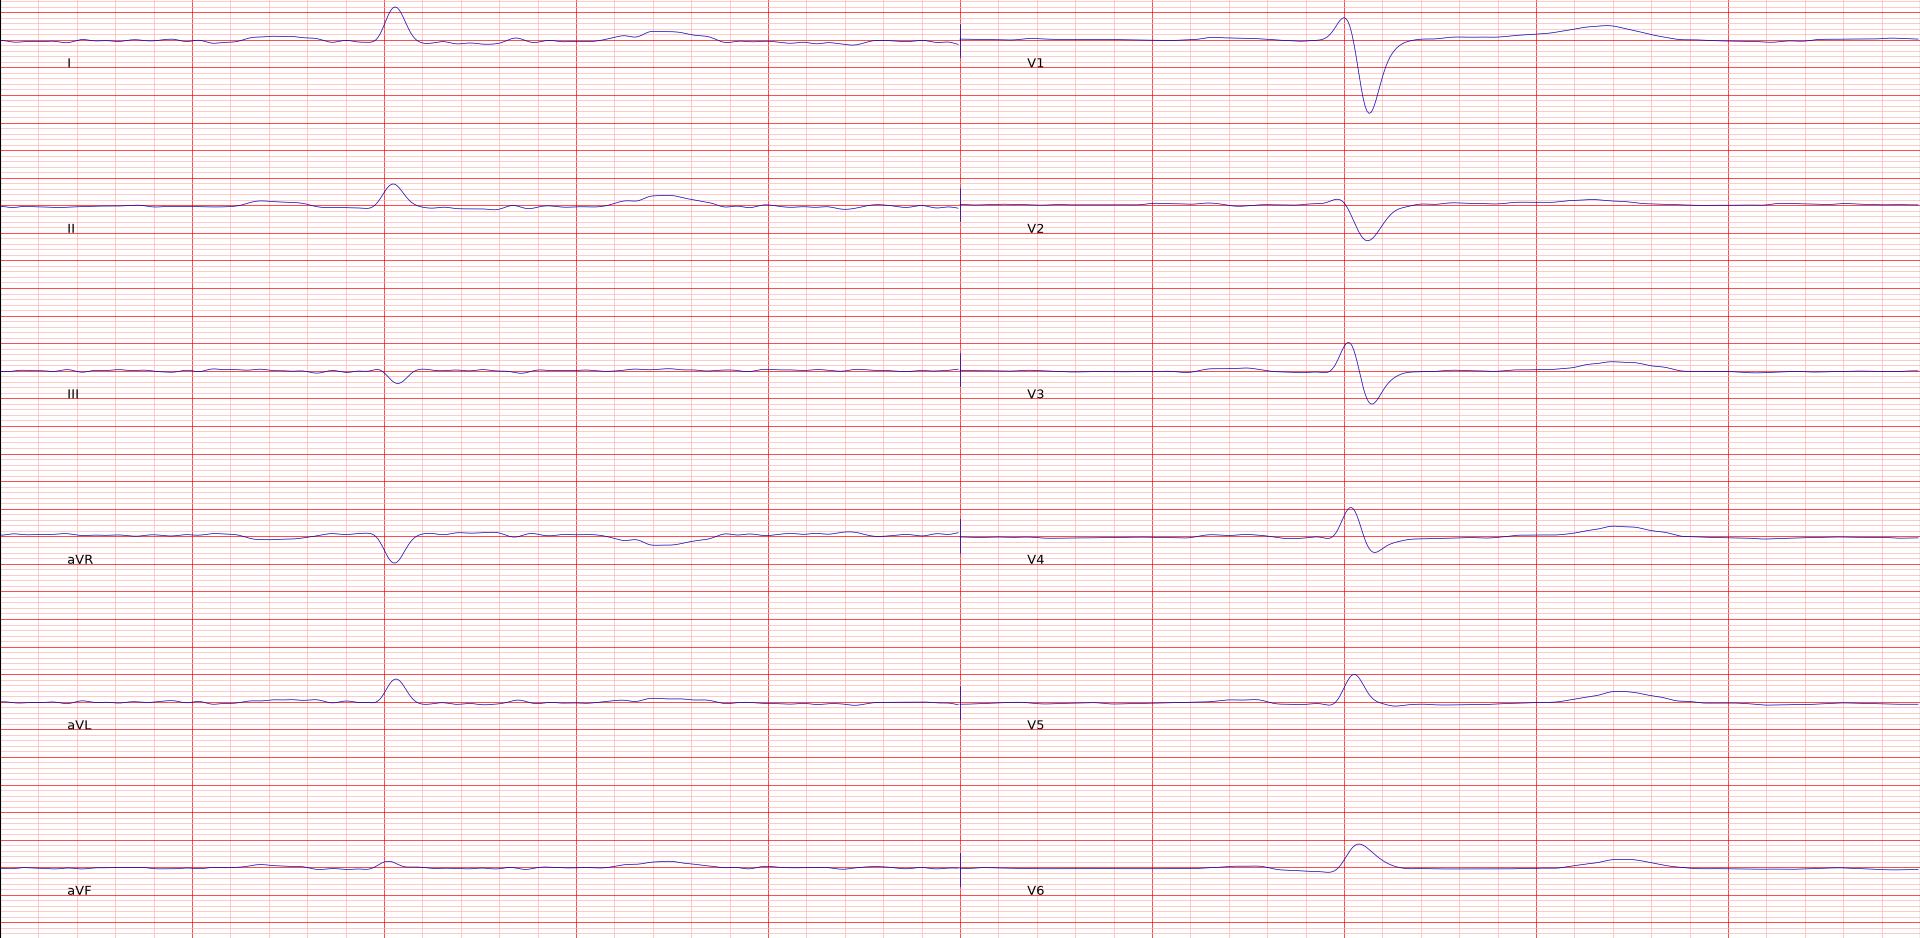
\includegraphics[width=\textwidth]{images/misplace_ecg.png}
	\caption{Battito trasformato secondo lo scambio RA--LA.}
	\label{fig:scambio_RA_LA}
\end{figure}
\newpage

\subsection{Regole di generazione del dataset finale}
\label{final_dataset}
L'applicazione pratica delle trasformazioni descritte sopra ai battiti segmentati segue alcune regole progettuali, motivate dalla necessità di produrre un dataset privo di possibili fonti di \emph{data leakage}. Tali regole si applicano ai soli split di training e validazione, gli unici in cui viene simulato il malposizionamento (si veda la Sezione~\ref{sec:beat_count_per_split} per il test).

\begin{enumerate}
	\item \textbf{I due battiti di ogni registrazione hanno etichette diverse.} Per ciascuna registrazione di training o validazione vengono estratti due segmenti, come descritto nella Sezione~\ref{beat-by-beat-segmentation}, e a ciascuno dei due viene assegnata un'etichetta diversa dall'altro, scelta tra ``normale'' e le diverse tipologie di scambio selezionate, secondo proporzioni configurabili. Questa scelta è motivata dal fatto che assegnare la stessa etichetta a entrambi i battiti di una stessa registrazione non aggiungerebbe reale informazione che la rete possa apprendere, finendo per appesantire la fase di training senza alcun guadagno.
	\item \textbf{Per ciascun battito viene mantenuta una sola versione.} Il dataset finale non contiene, per uno stesso segmento originale, sia la versione acquisita correttamente sia quella trasformata: viene conservata esclusivamente la versione corrispondente alla classe assegnata. In questo modo si evita di introdurre nel dataset coppie di esempi quasi identici (differenti unicamente per l'etichetta), che comprometterebbero la validità dello split e potrebbero facilitare un apprendimento per memorizzazione anziché per generalizzazione.
	\item \textbf{L'assegnazione delle classi avviene sull'insieme combinato PTB-XL + Georgia di ciascuno split.} Le etichette non vengono assegnate separatamente ai battiti dei due database, ma sull'unione di tutte le registrazioni PTB-XL e Georgia appartenenti allo stesso split (training o validazione): questo garantisce che le proporzioni tra classi richieste in fase di configurazione (ad esempio 50\% ``normale'' e il resto suddiviso equamente tra i quattro tipi di scambio) valgano sul dataset combinato effettivamente usato per addestrare il modello, e non separatamente sulle due sorgenti.
	\item \textbf{Lo split tra training, validazione e test è definito a monte, per paziente.} Come descritto nella Sezione~\ref{sec:split}, la suddivisione avviene prima della segmentazione ed è basata sull'identificativo di paziente: questo garantisce che tutti i battiti provenienti da uno stesso paziente appartengano a un unico insieme, evitando che il modello venga valutato su battiti provenienti da un paziente già osservato, seppur in forma diversa, durante l'addestramento.
\end{enumerate}

\section{Struttura del dataset finale}
\label{sec:struttura_finale}

Al termine della pipeline, il dataset è organizzato in tre sottocartelle separate, una per ciascuno split (\texttt{train/}, \texttt{val/}, \texttt{test/}), ciascuna con la stessa struttura interna:

\begin{itemize}
	\item una cartella \texttt{segments/}, contenente un file \texttt{.npy} per ciascun battito, con forma \texttt{(12, lunghezza\_finestra)}, cioè \emph{leads-first}, con le 12 derivazioni sulla prima dimensione, dove \texttt{lunghezza\_finestra} dipende dalla frequenza di campionamento scelta (500 campioni per una finestra di un secondo a \SI{500}{Hz}).
	\item un file di indice: \texttt{final\_dataset\_index.csv} per gli split di training e validazione, \texttt{beats\_index.csv} per lo split di test. In entrambi i casi, ogni riga corrisponde a un battito e riporta: il nome del file \texttt{.npy} corrispondente (\texttt{filename}); l'identificativo della registrazione di provenienza, prefissato con la sorgente (\texttt{ecg\_id}, ad es. \texttt{ptbxl\_1234} o \texttt{georgia\_E00001}); l'identificativo del paziente, anch'esso prefissato con la sorgente (\texttt{patient\_id}); il database di origine (\texttt{source}, \texttt{ptbxl} oppure \texttt{georgia}); la posizione del battito all'interno della registrazione (\texttt{beat\_idx\_in\_record}); il campione in cui è stato rilevato il picco R utilizzato per la segmentazione (\texttt{r\_peak\_sample}); e l'etichetta di classe (\texttt{label}: \texttt{normal} oppure il tipo di scambio simulato -- per il test, sempre \texttt{normal});
	\item un file \texttt{skipped\_records.csv}, che elenca le registrazioni scartate durante l'elaborazione di quello split, con il relativo motivo (ad esempio segnale contenente valori non definiti, numero di picchi R insufficiente, o errori di lettura/formato del file WFDB).
\end{itemize}

Questa struttura, oltre a facilitare il caricamento efficiente dei dati durante l'addestramento (ogni esempio può essere letto individualmente, senza necessità di caricare l'intero dataset in memoria), consente di ricostruire in ogni momento la provenienza di ciascun esempio, e mantiene traccia delle registrazioni escluse dalla pipeline, utile in fase di verifica della qualità del dataset. La distinzione tra i due file di indice (\texttt{final\_dataset\_index.csv} e \texttt{beats\_index.csv}) riflette inoltre la diversa natura dei due split: mentre train e validazione sono pensati per l'addestramento a livello di singolo battito, il test è organizzato per essere valutato a livello di intera registrazione tramite \emph{majority voting} su tutti i suoi battiti, aggregati tramite la colonna \texttt{ecg\_id}.

\section{Terzo database solo per il test}
\label{china_dataset}

Oltre allo split di test ricavato da PTB-XL e Georgia (Sezione~\ref{sec:beat_count_per_split}), le prestazioni del modello sono state valutate anche su un \textit{terzo database, indipendente e utilizzato esclusivamente per il test}, con l'obiettivo di verificare la capacità di generalizzazione su registrazioni provenienti da un contesto di acquisizione completamente diverso da quello visto in fase di addestramento (diversa popolazione, apparecchiatura e origine geografica).

Il database in questione, indicato nella repository del progetto come \emph{China database}, corrisponde all'\emph{ECG Arrhythmia Database} distribuita da PhysioNet~\cite{zheng2022ecgarrhythmia}, nota in letteratura anche come database Chapman--Shaoxing--Ningbo (CSN)~\cite{zheng2020chapman}. Si tratta di un database di ECG a 12 derivazioni raccolto in Cina, la cui popolazione, apparecchiatura di acquisizione e condizioni di registrazione differiscono sensibilmente da quelle di PTB-XL e Georgia.

\subsection{Preparazione dei dati}

Il database originale contiene 45\,152 registrazioni ECG. Durante la fase di preparazione, ogni registrazione è stata convertita in un insieme di segmenti con la stessa procedura di segmentazione descritta nella Sezione~\ref{beat-by-beat-segmentation} per lo split di test di PTB-XL e Georgia..

Delle 45\,152 registrazioni originali, 43\,712 sono state elaborate con successo, mentre 1\,440 sono state escluse a causa dell'assenza di picchi R rilevabili, di segmenti validi ai bordi del segnale, oppure di errori durante il caricamento o il preprocessing (le stesse categorie di scarto già introdotte per PTB-XL e Georgia nella Sezione~\ref{sec:struttura_finale}). Dalle registrazioni utilizzabili sono stati estratti complessivamente 445\,520 battiti. Le caratteristiche principali del database e i risultati della fase di preparazione sono riassunti nella Tabella~\ref{tab:china_caratteristiche}.

\begin{table}[htbp]
	\centering
	\caption{Caratteristiche principali del database utilizzato esclusivamente per il test (China)~\cite{zheng2022ecgarrhythmia, zheng2020chapman}.}
	\label{tab:china_caratteristiche}
	\begin{tabular}{@{}ll@{}}
		\toprule
		\textbf{Caratteristica} & \textbf{Valore} \\
		\midrule
		Numero di registrazioni ECG originali & 45\,152 \\
		Registrazioni elaborate con successo & 43\,712 \\
		Registrazioni escluse & 1\,440 \\
		Battiti estratti & 445\,520 \\
		Durata di ciascuna registrazione & 10 secondi \\
		Derivazioni & 12 \\
		Frequenza di campionamento & 500~Hz \\
		Formato dei segnali grezzi & WFDB \\
		Annotazioni diagnostiche & Codici SNOMED-CT \\
		Origine geografica & Cina (interferenza a \SI{50}{Hz}) \\
		Ruolo nella pipeline & solo test, nessuna trasformazione simulata \\
		\bottomrule
	\end{tabular}
\end{table}

\subsection{Utilizzo nella valutazione}

A differenza degli split di training e validazione, sui battiti estratti dal database China non è stata applicata alcuna trasformazione artificiale di malposizionamento, tutti i battiti sono etichettati come \texttt{normal}, coerentemente con l'assunzione, già discussa per PTB-XL e Georgia, che le registrazioni pubbliche disponibili siano state acquisite con un posizionamento corretto degli elettrodi.

Questa scelta consente di misurare sul database China, la capacità di generalizzare su un contesto di acquisizione mai osservato durante il training. Come per lo split di test di PTB-XL e Georgia, anche in questo caso la valutazione non è condotta a livello del singolo battito, ma le predizioni relative ai diversi segmenti appartenenti alla stessa registrazione vengono aggregate tramite \emph{majority voting}, ottenendo una predizione finale a livello di intera registrazione. Questa aggregazione riduce l'influenza di eventuali errori su singoli battiti isolati e permette di dare una migliore valutazione della capacità del modello di riconoscere la eventuali malposizionamenti.